\documentclass[12pt,english,dvipsnames,aspectratio=169,handout]{beamer}\usepackage[]{graphicx}\usepackage[]{xcolor}
% maxwidth is the original width if it is less than linewidth
% otherwise use linewidth (to make sure the graphics do not exceed the margin)
\makeatletter
\def\maxwidth{ %
  \ifdim\Gin@nat@width>\linewidth
    \linewidth
  \else
    \Gin@nat@width
  \fi
}
\makeatother

\definecolor{fgcolor}{rgb}{0.345, 0.345, 0.345}
\newcommand{\hlnum}[1]{\textcolor[rgb]{0.686,0.059,0.569}{#1}}%
\newcommand{\hlstr}[1]{\textcolor[rgb]{0.192,0.494,0.8}{#1}}%
\newcommand{\hlcom}[1]{\textcolor[rgb]{0.678,0.584,0.686}{\textit{#1}}}%
\newcommand{\hlopt}[1]{\textcolor[rgb]{0,0,0}{#1}}%
\newcommand{\hlstd}[1]{\textcolor[rgb]{0.345,0.345,0.345}{#1}}%
\newcommand{\hlkwa}[1]{\textcolor[rgb]{0.161,0.373,0.58}{\textbf{#1}}}%
\newcommand{\hlkwb}[1]{\textcolor[rgb]{0.69,0.353,0.396}{#1}}%
\newcommand{\hlkwc}[1]{\textcolor[rgb]{0.333,0.667,0.333}{#1}}%
\newcommand{\hlkwd}[1]{\textcolor[rgb]{0.737,0.353,0.396}{\textbf{#1}}}%
\let\hlipl\hlkwb

\usepackage{framed}
\makeatletter
\newenvironment{kframe}{%
 \def\at@end@of@kframe{}%
 \ifinner\ifhmode%
  \def\at@end@of@kframe{\end{minipage}}%
  \begin{minipage}{\columnwidth}%
 \fi\fi%
 \def\FrameCommand##1{\hskip\@totalleftmargin \hskip-\fboxsep
 \colorbox{shadecolor}{##1}\hskip-\fboxsep
     % There is no \\@totalrightmargin, so:
     \hskip-\linewidth \hskip-\@totalleftmargin \hskip\columnwidth}%
 \MakeFramed {\advance\hsize-\width
   \@totalleftmargin\z@ \linewidth\hsize
   \@setminipage}}%
 {\par\unskip\endMakeFramed%
 \at@end@of@kframe}
\makeatother

\definecolor{shadecolor}{rgb}{.97, .97, .97}
\definecolor{messagecolor}{rgb}{0, 0, 0}
\definecolor{warningcolor}{rgb}{1, 0, 1}
\definecolor{errorcolor}{rgb}{1, 0, 0}
\newenvironment{knitrout}{}{} % an empty environment to be redefined in TeX

\usepackage{alltt}
\usepackage{fontspec}
\setsansfont[Mapping=tex-text]{Fira Sans}
\setcounter{secnumdepth}{4}
\setcounter{tocdepth}{4}
\usepackage[normalem]{ulem}
\usepackage[T1]{fontenc}
\usepackage{dcolumn}
\usepackage{booktabs}
\usepackage{bm}
\usepackage{setspace}
\makeatletter
\usetheme{metropolis}
\setbeamertemplate{frame footer}{Bosancianu | Schaub | Hertie School}
\setbeamerfont{page number in head/foot}{size=\tiny}
\setbeamercolor{footline}{fg=gray}
\usepackage{xcolor}
\setbeamercovered{transparent}
\usepackage{tikz}
\usetikzlibrary{arrows, positioning, fit, shapes, shapes.misc}
\usepackage[labelformat=empty]{caption}
% For table captions in Beamer
\usepackage[sectionbib]{apacite}
\renewcommand{\bibliographytypesize}{\footnotesize}
\makeatletter
\let\st@rtbibsection\@bibnewpage
\let\st@rtbibchapter\@bibnewpage
\makeatother
\usepackage{amsmath, mathtools}
\usepackage{xunicode}
\usepackage{hyperref}
\graphicspath{{./figures/}} 
% Defines a checkmark
\def\checkmark{\tikz\fill[scale=0.4,color=orange](0,.35) -- (.25,0) -- (1,.7) -- (.25,.15) -- cycle;}
% Code for circles in Table cells
\newcounter{nodemarkers}
\newcommand\circletext[1]{%
    \tikz[overlay,remember picture] 
        \node (marker-\arabic{nodemarkers}-a) at (0,1.5ex) {};%
    #1%
    \tikz[overlay,remember picture]
        \node (marker-\arabic{nodemarkers}-b) at (0,0){};%
    \tikz[overlay,remember picture,inner sep=2pt]
        \node[draw,ellipse,fit=(marker-\arabic{nodemarkers}-a.center) (marker-\arabic{nodemarkers}-b.center)] {};%
    \stepcounter{nodemarkers}%
}
% wide itemize and enumerate
\newenvironment{wideitemize}{\itemize\addtolength{\itemsep}{.3em}}{\enditemize}
\newenvironment{wideenumerate}{\enumerate\addtolength{\itemsep}{.3em}}{\endenumerate}
% boxes
\def\boxitorange#1{%
  \smash{\color{orange}\fboxrule=1pt\relax\fboxsep=2pt\relax%
  \llap{\rlap{\fbox{\vphantom{0}\makebox[#1]{}}}~}}\ignorespaces
}
\def\boxitblue#1{%
  \smash{\color{blue}\fboxrule=1pt\relax\fboxsep=2pt\relax%
  \llap{\rlap{\fbox{\vphantom{0}\makebox[#1]{}}}~}}\ignorespaces
}
\newcommand{\indep}{\perp \!\!\!\! \perp}
\setbeamertemplate{itemize items}{\checkmark}
\usepackage{multirow}
\hypersetup{pdfauthor={Bosancianu and Schaub},
	pdftitle={Statistical Modeling and Causal Inference with R},
	pdfsubject={Week 6: Matching},
	pdfkeywords={Berlin, Hertie, 2020, week 5}}
\title{\textsc{Statistical Modeling and Causal Inference with R}}
\subtitle{Week 6: Matching}
\date{October 12, 2020}
\author{Manuel Bosancianu \hfill Max Schaub}
\institute{Hertie School of Governance}
\IfFileExists{upquote.sty}{\usepackage{upquote}}{}
\begin{document}
\maketitle


\begin{frame}
	\frametitle{Today's focus}
	\begin{itemize}
		\item Subclassification: the mother of all matching methods
		\item Matching metrics and their application
		\item Common matching algorithms
	\end{itemize}
\end{frame}


\section{Subclassification: the mother of all matching methods}


\begin{frame}
  \frametitle{Subclassification and the independence assumption}
\footnotesize
Data from study on internet use (0,1) on right-wing support (0,1), n=100


\tiny
\begin{table}\centering
\begin{tabular}{l*{1}{lccc}}
\toprule
Raw numbers                                  &         &         &         \\
\midrule
Internet use
                                             &\multicolumn{3}{c}{Right-wing support} \\
                                             &     yes&       no&      total    \\
yes                                          &      40&       33&         73     \\
no                                           &      11&       16&         27     \\
\hline
\hline
                                       &         &         &         \\
Shares                                 &         &         &         \\
\midrule
Internet use
                                             &\multicolumn{3}{c}{Right-wing support} \\
yes                                          &    0.55&           &             \\
no                                           &    0.41&           &             \\
\bottomrule
\end{tabular}
\caption{\scriptsize Data on internet use and right-wing support (simulated)}
\end{table}

\footnotesize
$NATE = E[Y_{1i}|D_i=1] - E[Y_{0i}|D_i=0] = 0.55-0.41 = \textcolor{orange}{0.14}$

\end{frame}



\begin{frame}
  \frametitle{Subclassification as an answer to confounding}
\footnotesize
But what about confounders, for example the age of the respondent?

\vspace{15mm}
	\begin{figure}
		\centering
		\scriptsize
		\begin{tikzpicture}[->,
			>=stealth',
			shorten >=1pt,
			auto,
			thick]
			\draw[fill=black, draw=black] (0,0) circle (0.8ex) node (a) [below, yshift=-0.2cm] {\scriptsize{$D_i$ Internet use}};
			\draw[fill=black, draw=black] (2,0) circle (0.8ex) node (b) [below, yshift=-0.2cm] {\scriptsize{$Y_i$ RW-support}};
			\draw[fill=black, draw=black] (1,1.5) circle (0.8ex) node (b) [above, yshift=0.2cm] {\scriptsize{$W_i$, e.g.\ Age}};
			\draw[->, black] (0,0) -- (1.92,0);
			\draw[<-, black] (1,1.4) -- (0,0.08);
			\draw[->, black] (1,1.5) -- (1.94,0.06);
		\end{tikzpicture}
	\end{figure}\bigskip

\vspace{15mm}
\end{frame}



\begin{frame}
  \frametitle{Subclassification as an answer to confounding}
\footnotesize
Looking at the share of internet users by age group, we can observe stark differences.


\tiny
\begin{table}\centering
\begin{tabular}{lc}
\toprule
\multicolumn{2}{c}{Share internet users by age} \\
\midrule
Aged 20-40                                          &    0.9    \\
Aged 41-60                                          &    0.8    \\
Aged 60+                                            &    0.5    \\
\bottomrule
\end{tabular}
\end{table}

\footnotesize
Thus, the treatment is clearly not independent of age -- the independence assumption $Y_{i0},Y_{i1} {\indep} D_i$ is violated.

\end{frame}



\begin{frame}
  \frametitle{Subclassification as a way to create conditional independence}
\footnotesize

From previous weeks we know that we can condition on a known confounder to close the back door path.

In other words, we can make use of the \emph{conditional} independence assumption (CIA): $Y_{i0},Y_{i1} {\indep} D_i|W_i$.

One way of doing this is by using a regression model in the form $Y_i = \alpha + \beta D_i + \gamma W_i + u_i$.

We derived mathematically how regression can be used to control for confounders. 

Here we will discuss other methods to achieve the same result.

\end{frame}




\begin{frame}
  \frametitle{Looking for twins}
\footnotesize

Rather than invoking regression mechanics to achieve \emph{ceteris paribus}, we start more simply: by comparing like and like.

The aim is to \textcolor{orange}{find units that are similar in all respects but the treatment}. We are looking for twins that are identical in all respects save for the fact that one received the treatment, but the other did not.

A first, most simple method is subclassification. The idea is to split our sample in strata of the potential confounder, and then to only compare treatment effects \emph{within} these strata. Consider our example:

\tiny
\begin{table}\centering
\begin{tabular}{l*{1}{lccc}}
\toprule
Raw numbers                                  &         &         &         \\
\midrule
Internet use
                                             &\multicolumn{3}{c}{Right-wing support} \\
                                             &     yes&       no&      total    \\
yes                                          &      40&       33&         73     \\
no                                           &      11&       16&         27     \\
\bottomrule
\end{tabular}
\end{table}

\end{frame}




\begin{frame}
  \frametitle{Conditioning using subclassification}
\footnotesize

Subclassification gives us the following frequency table:

\tiny
\begin{table}\centering
\begin{tabular}{@{\extracolsep{7pt}}l*{6}{c}@{}}
\toprule
\multicolumn{7}{l}{Numbers of right-wing supporters by internet use and age class}      \\
\midrule
Internet use
                &\multicolumn{2}{c}{Aged 20--40} &\multicolumn{2}{c}{Aged 41--60} &\multicolumn{2}{c}{Aged 60+} \\
                &\multicolumn{2}{c}{Right-wing support} &\multicolumn{2}{c}{Right-wing support} &\multicolumn{2}{c}{Right-wing support} \\
\cmidrule(l){2-3}
\cmidrule(l){4-5}
\cmidrule(l){6-7}
                &     yes&     total  &     yes&     total&     yes&     total \\
yes             &       9&     18     &      28&        40&       3&       15  \\
no              &       1&      2     &       7&        10&       3&       15  \\
\hline
\hline
\rule{0pt}{4ex}
Shares   &         &         &         \\
\midrule
yes             &       0.5&      &      0.7&       &       0.2&         \\
no              &       0.5&      &      0.7&       &       0.2&         \\

\bottomrule
\end{tabular}

\end{table}

\scriptsize 
This allows us to compare rightwing support for individuals aged 20-40 that use and do not use the internet, for individuals aged 41-60 that use and do not use the internet, \ldots

We can see that when comparing right-wing support between `treated' and `untreated' units, the shares of right-wing supporters are actually identical  within each of the three age-subgroups!

\end{frame}




\begin{frame}
  \frametitle{Conditioning using subclassification}
\footnotesize
In other words, $NATE_{20-40} = NATE_{41-60} = NATE_{60+} = 0$.

\footnotesize
It follows (in this example) that the weighted overall, adjusted NATE is also zero: 

$NATE_{overall} = NATE_{20-40}\times\frac{20}{100} + NATE_{41-60}\times\frac{50}{100} + NATE_{60+}\times\frac{30}{100} = 0$.$^*$

\vspace{25mm}

\scriptsize
$^*$ Note that the same result could be recovered with a regression model in the form $\text{RW-support} = \alpha + \beta \text{InternetUse} + \gamma_1 \text{Age}_{41-61} + \gamma_2 \text{Age}_{61+}+ u_i$.

\end{frame}



\begin{frame}
  \frametitle{Conditioning using subclassification}
\footnotesize

By subclassifying our data into strata and assuming that age is the only confounder we have satisfied the backdoor criterion, and $NATE_{overall}$ estimates the $ATE$. The estimated effect of internet on right-wing voting is zero. 

But what about other confounders, e.g.\ gender, which is also plausibly related to internet usage and right-wing attitudes?

How can we use subclassification be used to condition on this second variable?

\vspace{3cm}

\end{frame}


\begin{frame}
  \frametitle{Subclassification with many dimensions}
\footnotesize
Introducing another dimension along which to classify increases the number of cells to consider twofold. There are now $2\times 3 \times 2=12$ cells (of which 8 are shown in the table):

\tiny
\begin{table}\centering
\begin{tabular}{@{\extracolsep{7pt}}l*{9}{c}@{}}
\toprule
\multicolumn{7}{l}{Numbers of right-wing supporters by age class and gender}  &       &         &         \\
\midrule
Internet use & & & & & & & & & \\
                &\multicolumn{4}{c}{Aged 20--40} &\multicolumn{4}{c}{Aged 41--60} &\ldots \\
                &\multicolumn{2}{c}{Male} &\multicolumn{2}{c}{Female} &\multicolumn{2}{c}{Male} &\multicolumn{2}{c}{Female} & \ldots  \\
                &\multicolumn{2}{c}{RW-support} &\multicolumn{2}{c}{RW-support} &\multicolumn{2}{c}{RW-support} &\multicolumn{2}{c}{RW-support} & \ldots \\
\cmidrule(l){2-5}
\cmidrule(l){6-9}
                &     yes&     total  &     yes&     total&     yes&     total &     yes&     total  & \ldots \\
yes             &       2&      5     &      2&          4&       15&       23&      10&       17   & \ldots \\
no              &    \circletext{\textcolor{orange}{--}}&      \circletext{\textcolor{orange}{--}}    &      1&          1&        2&        5&       10&       10   & \ldots \\
\bottomrule
\end{tabular}
\end{table}

\footnotesize
There are several noteworthy observations in this table.

\end{frame}


\begin{frame}
  \frametitle{The curse of dimensionality}
\footnotesize

Already with this limited number of dimensions, we run into trouble! Note the circled cells:

There are no men aged 20--40 that do not use the internet! The respective cells are not populated. In other words, there are no observations that are equal with regard to gender and age that we can compare these men to. They lack a counterfactual.

This is the \emph{curse of dimensionality} biting -- the more variables we try to condition, the more cells we create, and the more likely it becomes that -- with limited sample size -- cells will not be populated.

If we wanted to control for additional variables like education, the problem would worsen. We would now need to create a table with $2\times 3 \times 2 \times 3=36$ cells -- of which many would surely be empty.

\end{frame}



\begin{frame}
  \frametitle{Common support (and lack thereof)}
\footnotesize

With such missing data, our subclassification scheme is no longer fully defined. 

We say that the problematic cells lack \textcolor{orange}{common support}.

Common support requires that for each strata, there exist observations in both the treatment and control group.

Without common support, we cannot calculate the group-specific treatment effects, and the ATE can no longer be estimated.

While subclassification therefore in principle allows for establishing conditional independence, its application is limited to simple cases. 

\end{frame}


\begin{frame}
  \frametitle{One-sided lack of common support and the ATT}
\footnotesize

It matters which information is missing. Once any cell is not fully populated, we can no longer use subclassification to estimate the ATE.

However, as long as we have populated cells in the control condition, we can still estimate the average treatment effect for the treated, the $ATT= E[Y_{1i}|D_i=1] - E[Y_{0i}|D_i=1]$. 

Because estimating the ATT requires less complete data, estimating the ATT is often more feasible, especially in cases where you have few treatment observations, but many control observations.

However, in our example, a control cell is empty. In this case, subclassification is `broken'.

\vspace{1cm}

\end{frame}


\section{Matching metrics and their application}



\begin{frame}
  \frametitle{Matching philosophy}
\footnotesize

Matching techniques losen the requirement that each cell should have counterfactual in the respective control cell.

Instead, matching algorithms try to find \textcolor{orange}{the most plausible counterfactual within the data} for a given observation in a treatment cell.

Where exact control cells are available, these exact matches will usually be chosen. 

Where this is not the case, matching algorithms \textcolor{orange}{minimize some metric defining the distance between treatment and control cells}, and choose control units that are closest to a given treatment unit lacking an exact match.

If there is more than one matched unit at the same distance, matching algorithms usually use the \textcolor{orange}{average of all matched units}.


\end{frame}




\begin{frame}
  \frametitle{Choosing the best counterfactual}
\scriptsize
In our original example, we might for example match the young, internet-using men who lack a direct counterfactual (marked in orange) with a) women of the same age group, or b) men aged 41-60 (both marked in blue).

\tiny
\begin{table}\centering
\begin{tabular}{@{\extracolsep{7pt}}l*{9}{c}@{}}
\toprule
\multicolumn{7}{l}{Numbers of right-wing supporters by age class and gender}  &       &         &         \\
\midrule
Internet use & & & & & & & & & \\
                &\multicolumn{4}{c}{Aged 20--40} &\multicolumn{4}{c}{Aged 41--60} &\ldots \\
                &\multicolumn{2}{c}{Male} &\multicolumn{2}{c}{Female} &\multicolumn{2}{c}{Male} &\multicolumn{2}{c}{Female} & \ldots  \\
                &\multicolumn{2}{c}{RW-support} &\multicolumn{2}{c}{RW-support} &\multicolumn{2}{c}{RW-support} &\multicolumn{2}{c}{RW-support} & \ldots \\
\cmidrule(l){2-5}
\cmidrule(l){6-9}
                &     yes&     total  &     yes&     total&     yes&     total &     yes&     total  & \ldots \\
yes             &       \circletext{\textcolor{orange}{2}}&      \circletext{\textcolor{orange}{5}}     &      2&          4&       15&       23&      10&       17   & \ldots \\
no              &    --&      --    &      \circletext{\textcolor{blue}{1}}&          \circletext{\textcolor{blue}{1}}&        \circletext{\textcolor{blue}{2}}&        \circletext{\textcolor{blue}{5}}&       10&       10   & \ldots \\
\bottomrule
\end{tabular}
\end{table}

\scriptsize
Both are plausible counterfactuals that are `one step away'. 

Matching algorithms will usually determine which of the two dimensions -- gender or age -- should be given more weight in the distance matrix, and will choose the match accordingly.

Or they will define some virtual counterfactual that mixes the outcomes for both plausible matching cells.

\end{frame}



\begin{frame}
  \frametitle{Basic matching estimators}
\footnotesize

Let's look again, in a more technical way, at the estimands that we are typically trying to recover from the data: the ATT, and the ATE, and how matching tries to approximate them.

As mentioned, the difference between the ATT and ATE from a matching perspective is that for the ATT, we only need to find counterfactuals for the treated units, while for the ATE, we also need counterfactuals for control units with missing treatment matches \cite[119]{cunningham_causal_2021}.

\vspace{3cm}

\end{frame}


\begin{frame}
  \frametitle{Basic matching estimators}
\footnotesize

The matching estimator for the ATT is 

\begin{equation*} \displaystyle
\hat{\delta}_{ATT} = \frac{1}{N_T}\sum_{D_{i}=1}(Y_i - Y_{j(i)}) = \frac{1}{N_T} \sum_{D_{i}=1}(Y_i - [\frac{1}{M}\sum_{D_{i}=1}Y_{j_{m}(i)})
\end{equation*} \footnotesize

That is, our estimate for the ATT is the difference between the outcomes $Y_i$ of all $N_T$ treated units minus the outcome for the matched closest units $Y_{j(i)}$

If there is more than one match, the average oucome of the matched units \emph{s} is used as a counterfactual. That's what the term $\frac{1}{M}\sum_{D_{i}=1}Y_{j_{m}(i)}$ means.

\vspace{3cm}

\end{frame}



\begin{frame}
  \frametitle{Basic matching estimators}
\footnotesize

The matching estimator for the ATE is 

\begin{equation*} \displaystyle
\hat{\delta}_{ATE} = \frac{1}{N}\sum_{i=1}^{N}(2D_i-1)(Y_i - Y_{j(i)}) =\frac{1}{N}\sum_{i=1}^{N}(2D_i-1)[Y_i - (\frac{1}{M} \sum_{D_{i}=1}Y_{j_{m}(i)})]
\end{equation*} \footnotesize

Different from the estimator for the ATT, this also finds matches for observations in the control condition, by having the term $2D_i-1$ be 1 if $D_i=1$ and -1 if $D_i=0$, which reversing the order of the outcomes.

\vspace{3cm}
\end{frame}


\section{Common matching algorithms}


\begin{frame}
  \frametitle{Common matching algorithms}
\footnotesize
There are many different matching techniques out there, and even more ways of implementing them. We here discuss three of the most fundamental and most widely used:

\begin{itemize}
\item Mahalanobis/nearest neighbor covariate matching
\item Propensity score matching
\item Coarsened exact matching
\end{itemize}

Another approach used in the social sciences is `genetic matching' \cite{diamond_genetic_2013}, and there also exists a whole universe of matching algorithms used for automated text analysis (e.g.\ based on the Levenshtein distance).
\end{frame}




\begin{frame}
  \frametitle{Mahalanobis/nearest neighbor covariate matching}
\footnotesize

As stated, most matching techniques minimize a metric of the distance between treatment and control cells and choose control units that are closest to a given treatment unit lacking an exact match.

The most simple metric that can be minimized is the Euclidean distance $||W_i - W_j||= \sqrt{\sum_{n=1}^{k} {(W_{ni}-W_{nj})}^2}$ -- the shortest path between two points in n-dimensional space, or the closely related Mahalanobis distance.

	 \begin{figure} 
    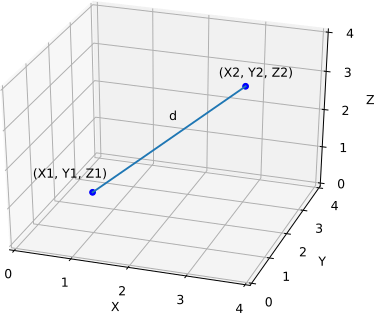
\includegraphics[height=.4\textheight,keepaspectratio=true]{../04-figures/06/01-euclidean}
    \end{figure}

\end{frame}


\begin{frame}
  \frametitle{Covariate matching in practice}
\footnotesize

In practice, when specifying a matching model, you will have to make have to make several decisions: 

\begin{itemize} \scriptsize
\item The number of matches allowed
\item The distance metric to use (e.g.\ Mahalanobis or Euclidean)
\item Sampling with replacement or without, i.e.\ whether the same unit can serve as a match for only one or several units.
\item Whether to enforce exact matching on some variables
\item Whether to use a \textcolor{orange}{caliper} -- a maximum distance between treated and control units beyond which units are declared `unmatchable', and are no further considered. The caliper defines which units are `on common support' -- here understood as reasonably close -- or `off common support' -- no close enough. The process of discarding units off common support is also called `trimming.'
\end{itemize}


How to make these decisions isn't fully defined, and a matter of trying out, reason, and experience. We will come back to practical aspects of matching towards the end.

\end{frame}


\begin{frame}
  \frametitle{Propensity score matching}
\footnotesize

Another very common metric used in matching (and other applications) is the \textcolor{orange}{propensity score}. 

The propensity score is defined as the probability of receiving the treatment given confounding variables:\\
Propensity score = $p(W) = Pr(D = 1|W)$.

Propensity score matching achieves a similar goal to nearest-neighbor matching on covariates, but in two steps steps. In a first step, all the potential confounder variables (that we usually refer to as $W$ here) are used to estimate a single value: the probability or propensity to receive a treatment.  

This is usually done with a maximum likelihood (logit or probit) model where we regress the treatment status $D_i$ on the covariates. The predicted outcome from this regression -- the predicted probability of receiving the treatment -- is the propensity score.

\end{frame}


\begin{frame}
  \frametitle{Propensity score matching}
\footnotesize

A typical model used for estimating the propensity score would take the form

$Pr(D = 1|W) = \Phi(\beta \bm{W})$

which describes a standard probit model. $\bm{W}$ here is the matrix with all potential confounders, and $\Phi$ is the cumulative distribution function of the standard normal distribution.

The \textcolor{orange}{propensity score theorem} holds that if the CIA $Y_{0},Y_{1} {\perp\!\!\!\perp} D|W$ applies, conditioning on the propensity score $p(W)$ will achieve conditional independence, i.e.\ $Y_{0},Y_{1} {\perp\!\!\!\perp} D|pr(W)$ (see: Cunningham \citeyear[143]{cunningham_causal_2021}).

\vspace{3cm}

\end{frame}



\begin{frame}
  \frametitle{Propensity score matching}
\footnotesize

The propensity score thus sums up, in a single number, all the information contained in the control variables that are needed to make the potential outcomes independent from the treatment status!$^*$

Instead of finding nearest neighbors with regard to all problematic covariates, we can find nearest neighbors in terms of the propensity score.

In so doing, all the practical issues mentioned above apply -- especially regarding the use of the caliper/trimming -- also apply here. 

We can also use the propensity score for weighing our data -- a method called inverse propensity score weighing (IPW).

\scriptsize $^*$ Note that this only holds, however, if your model for the estimating the propensity score is fully and correctly specified -- and only your DAG can tell you which variables to include \ldots

\end{frame}


\begin{frame}
  \frametitle{Plotting propensity scores}
\footnotesize
  
The propensity score gives you a single number with a very intuitive interpretation: the probability of receiving treatment given the covariates. 

It shows you how different treatment and control units in your data really are, and makes intuitively clear how much extrapolation your model will do. 

	 \begin{figure} 
    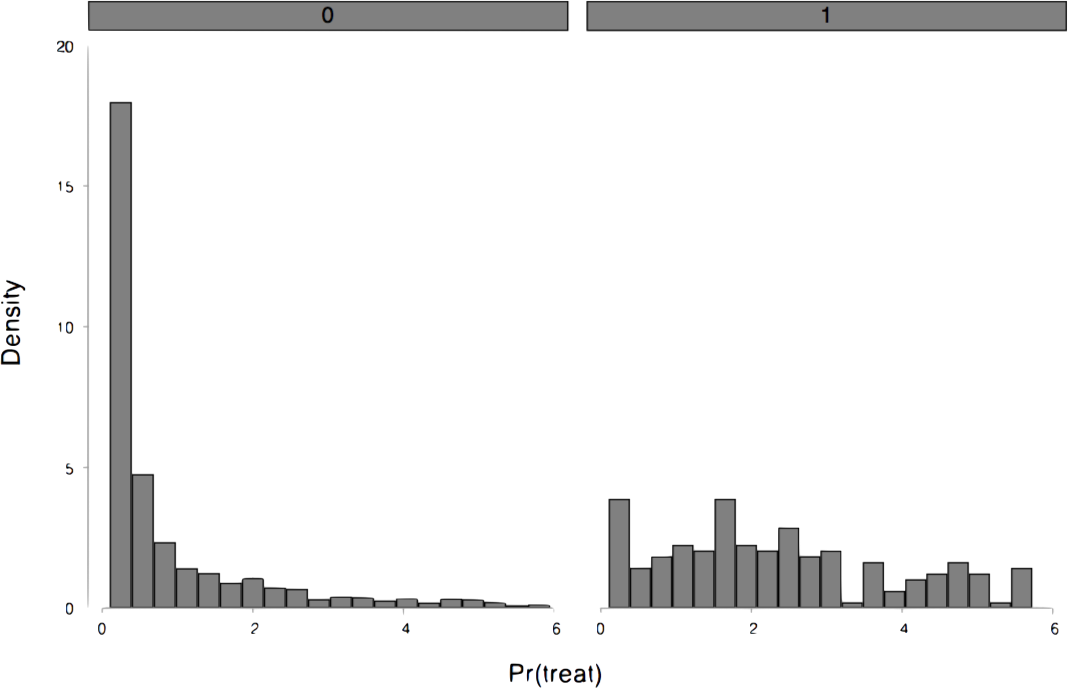
\includegraphics[height=.5\textheight,keepaspectratio=true]{../04-figures/06/02-hist_pscores_t}
    \end{figure}

\end{frame}



\begin{frame}
  \frametitle{A note on trimming}
\footnotesize

\textcolor{orange}{Trimming} -- discarding observations that are considered too different to have a plausible match in the data -- is one of the most powerful aspects of the matching process.

It sets the matching logic apart from other conditioning methods such as regression, which usually uses all the data, and tends to `create' counterfactuals even for observations that do not even have a `remote cousin' in the data.$^*$

It is by trimming that good balance on observable confounders can be achieved. A matched and trimmed dataset will often look like experimental data with regard to the observables (but of course not with regard to unobservables).

\scriptsize
$^*$ But note that many matching methods will do the same by default.

\end{frame}

\begin{frame}
  \frametitle{A note on trimming}
\footnotesize

The estimand that can be estimated after trimming, appliying a caliper, or otherwise changing the sample is therefore no longer the ATT or ATE, however.

Because we have changed our sample, what we are estimating is the \textcolor{orange}{local ATT} -- the the treatment effect averaged over only the subset of treated units for which good matches exist among available controls. 

\vspace{3cm}

\end{frame}


\begin{frame}
  \frametitle{Using the above matching techniques}
\scriptsize

The aim of a matching strategies discussed so far is to achieve balance on observable potential confounders. That is, after matching, the confounders should have the same average values in both the treatment and the control group.

In order to do so, in practice, several steps are taken (cp.\ Stuart \citeyear{stuart_matching_2010}):
\begin{enumerate}\scriptsize
\item Think carefully about the set of covariates to include in the matching procedure
\item Decide on the matching procedure (here assuming propensity score matching)
\item Specify the model used for matching, esp. the functional form of your covariariates (e.g.\ categorical, linear, quadratic, log), covariates to exactly match on, the maximum number of matches used to calculate the outcome etc.
\item Apply your matching algorithm
\item Inspect the propensity scores and consider common support: are the scores in treatment and control similar enough to justify using the whole sample/ estimate the ATT or ATE convincingly? If not, consider using a caliper.
\item Check your covariate balance in the matched sample. If balance is still poor, repeat steps 3 to 5.
\end{enumerate}

\end{frame}




\begin{frame}
  \frametitle{Coarsened exact matching}
\footnotesize
A final matching method that has gained a lot in popularity in recent years is \textcolor{orange}{coarsened exact matching} (CEM) \cite{iacus_causal_2012}.

Coarsened exact matching can be understood as a sophisticated form of subclassification. It proceeds in several steps:

\begin{enumerate} \scriptsize
\item In a first step covariates get split into temporary, coarse categories. For example, a continuous age variable might be split into three temporary age categories, while gender is split in two, and education in three categories. 
\item Second, matches between treatment and control units are found within overlapping strata -- just as in subclassification. 
\item  Third, data points that are alone in a class, i.e.\ that cannot be matched are `pruned' -- they are dropped from the data. Only treatment observations that have matches within their temporary strata are maintained. 
\item Finally, the temporary categories are removed, i.e.\ the original data remains unchanged. Just the information which units do or do not have matches within their strata is maintained.
\end{enumerate}

\end{frame}



\begin{frame}
  \frametitle{Coarsened exact matching}
\footnotesize

The pruned data set can then be analyzed with other statistical methods, like regression. 

Coarsened exact matching gives up on trying to maintain a full sample -- required to estimate ATT and ATE -- but instead prioritizes establishing covariance balance. 

CEM therefore paves the ground for estimating the \emph{local} ATT, similar to nearest-neighbor or propensity score approaches with a caliper.

The aim of CEM is to achieve balance without making assumptions on the fuctional form as to how the covariates influence treatment assigment -- a typical problem especially of propensity score matching.

\end{frame}



\begin{frame}
  \frametitle{Matching and regression}
\footnotesize

OLS regression can be seen as a matching technique that produces variance-weighted averages of treatment effects. See Angrist and Pischke \citeyear[54ff.]{angrist_mostly_2009} for details.

It is therefore not too different from nearest-neighbor covariate or propensity score matching.

Arguably the main difference between the use of regression and that of matching is in in terms of research culture/approach.

While regression is often used mindlessly, when using matching, scholars much more explicitly discuss issues such as the how covariates should enter the model and to what extent common support holds. 

If you practice the same care when specifying your regression model, the techniques will often give fairly similar results. 

Regression is also commonly used after coarsened exact matching to further reduce the impact of potential confounders.

\end{frame}



\begin{frame}
  \frametitle{Matching, regression, and IV}
\footnotesize

While subclassification, matching, and regression share many similarities, they are quite different from both the experimental method and instrumental variables.

In experiments and IV strategies, we use random assignment to treatment to take care of imbalance -- we are trying to create or isolate situations where the independence condition ($Y_{i0},Y_{i1} {\perp\!\!\!\perp} D_i$) holds.

With subclassification, matching, and regression techniques we attempt to \emph{explicity} balance the data. Rather than hoping for the independence assumption to hold thanks to (as-if) randomization, we are making our comparison work by invoking the \emph{conditional} independence assumption $Y_{i0},Y_{i1} {\perp\!\!\!\perp} D_i|W_i$.

Note that often these techniques are not mutually exclusive, but can (and often are) combined: in IV strategies, as-if random variation can be isolated \emph{conditional on controls} implemented with regression or matching. 

\end{frame}


% END
\begin{frame}
\begin{center}
    \LARGE Thank you for watching, and see you next Monday!
\end{center}
\end{frame}

% REFERENCES %

\begin{frame}[allowframebreaks]
\frametitle{References}
\bibliographystyle{apacite}
\scriptsize\bibliography{../Bibliography}
\end{frame}

\end{document}
